\begin{strip}
\centering
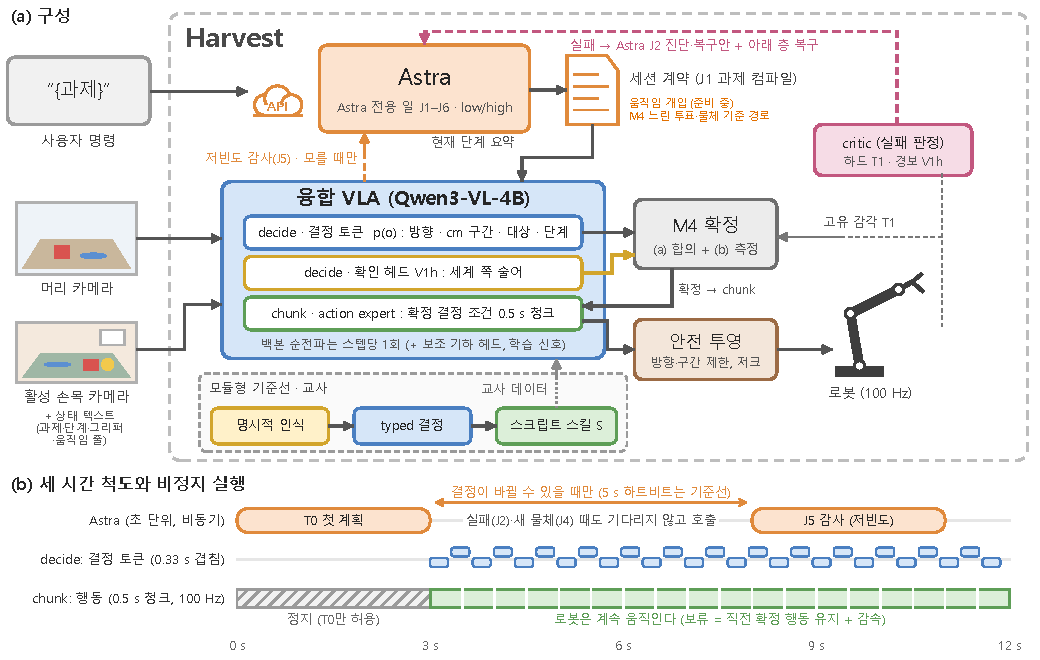
\includegraphics[width=\linewidth]{figures/overview.pdf}
\captionsetup{hypcap=false}
\captionof{figure}{\textbf{Harvest 개요.} 느린 상위 계획기 Astra가 세션 계약을 쓰고, 빠른 typed 결정 모델 Jev-L(로컬 GPU의 오픈 VLM을 보기 로그 확률로 쓰는 선택기)이 텍스트 상태와 머리 카메라 한 장을 받아 약 3\,Hz로 겹쳐 호출되며 스킬 안의 결정을 내린다. 겹친 결정은 확정 규칙(M4)을 거쳐 스킬이 100\,Hz로 실행한다. 작은 학습 보정기(R)는 Jev-L이 고른 방향과 크기 구간 안에서만 접근·접촉 근처의 잔차를 더하며, 결정 층(Astra, Jev-L)은 학습하지 않는다. 실패 판정은 코드 critic(M7) 한 곳에서만 내린다. Astra는 하트비트(잠정 5\,s)와 단계 경계에서도 비동기로 장면을 확인하고, 실패가 판정되면 연속 프레임(10장 격자)과 함께 비동기로 불린다. 그동안 로봇은 멈추지 않는다.}
\captionsetup{hypcap=true}
\label{fig:teaser}
\end{strip}
